%-------------------------------
%	PACKAGES AND OTHER DOCUMENT CONFIGURATIONS
%-------------------------------

% The \vref command specifies the location of the reference

%\documentclass[
%10pt, % Main document font size
%a4paper, % Paper type, use 'letterpaper' for US Letter paper
%oneside, % One page layout (no page indentation)
%twoside, % Two page layout (page indentation for binding and different headers)
%headinclude,footinclude, % Extra spacing for the header and footer
%BCOR5mm, % Binding correction
%]{scrartcl}


\documentclass{article}


%--------------------------------------------------------------
%	REQUIRED PACKAGES
%--------------------------------------------------------------

\usepackage[
nochapters, % Turn off chapters since this is an article        
beramono, % Use the Bera Mono font for monospaced text (\texttt)
%eulermath,% Use the Euler font for mathematics
pdfspacing, % Makes use of pdftex’ letter spacing capabilities via the microtype package
dottedtoc % Dotted lines leading to the page numbers in the table of contents
]{classicthesis} % The layout is based on the Classic Thesis style



\usepackage{arsclassica} % Modifies the Classic Thesis package

\usepackage[T1]{fontenc} % Use 8-bit encoding that has 256 glyphs

\usepackage[utf8]{inputenc} % Required for including letters with accents
%--------------------------------------------------------------
% Fonts and languages
\usepackage{libertinus} % The Libertinus font
%\usepackage[adobe-utopia]{mathdesign} % The Utopia font
%\usepackage[p,osf]{scholax}
% T1 and textcomp are loaded by package. Change that here, if you want
% load sans and typewriter packages here, if needed
%\usepackage{amsmath,amsthm}% must be loaded before newtxmath
% amssymb should not be loaded
%\usepackage[scaled=1.075,ncf,vvarbb]{newtxmath}% need to scale up math package
% vvarbb selects the STIX version of blackboard bold.


\usepackage[czech]{babel} % Český jazyk
%--------------------------------------------------------------
\usepackage{graphicx} % Required for including images
\graphicspath{{Figures/}} % Set the default folder for images

\usepackage{enumitem} % Required for manipulating the whitespace between and within lists

\usepackage{lipsum} % Used for inserting dummy 'Lorem ipsum' text into the template

\usepackage{subfig} % Required for creating figures with multiple parts (subfigures)

\usepackage{amsmath,amssymb,amsthm,amsfonts} % For including math equations, theorems, symbols, etc

\usepackage{varioref} % More descriptive referencing

\usepackage[top =3 cm, bottom = 3.5 cm, left = 1.5 cm, right = 1.5 cm]{geometry}

\usepackage{mathtools}

\usepackage{float}

\usepackage{caption}

%------------------------------------------------------------
%	DIAGRAMS AND TIKZ
\usepackage{smartdiagram}
\usepackage{metalogo}
\usepackage{tikz}
\usetikzlibrary{matrix,calc}

\usepackage{hhline} % kvůli double line v tabulkách
%------------------------------------------------------------
%	THEOREM STYLES
%------------------------------------------------------------

\theoremstyle{definition} % Define theorem styles here based on the definition style (used for definitions and examples)
\newtheorem{definition}{Definice}
\newtheorem{example}{Příklad}
\newtheorem{exercise}{Cvičení}

\theoremstyle{plain} % Define theorem styles here based on the plain style (used for theorems, lemmas, propositions)
\newtheorem{theorem}{Věta}

\theoremstyle{remark} % Define theorem styles here based on the remark style (used for remarks and notes)
\newtheorem{remark}{Poznámka}



%-------------------------------------------------------------
%	HYPERLINKS
%-------------------------------------------------------------

\hypersetup{
%draft, % Uncomment to remove all links (useful for printing in black and white)
colorlinks=true, breaklinks=true, bookmarks=true,bookmarksnumbered,
urlcolor=webbrown, linkcolor=RoyalBlue, citecolor=webgreen, % Link colors
pdftitle={}, % PDF title
pdfauthor={\textcopyright}, % PDF Author
pdfsubject={}, % PDF Subject
pdfkeywords={}, % PDF Keywords
pdfcreator={pdfLaTeX}, % PDF Creator
pdfproducer={LaTeX with hyperref and ClassicThesis} % PDF producer
}

 % Include the structure.tex file which specified the document structure and layout

%----------------------------------------------------
%	MATHEMATICS
%----------------------------------------------------

% Tělesa, obory íntegrity a metrické prostory
\newcommand{\C}{\mathbb{C}}
\newcommand{\R}{\mathbb{R}}
\newcommand{\N}{\mathbb{N}}
\newcommand{\Q}{\mathbb{Q}}
\newcommand{\Z}{\mathbb{Z}}
\renewcommand{\L}[2]{L^{#1} \left( #2 \right)} % Lebesgueovy prostory

\newcommand{\vc}[1]{\boldsymbol{#1}} % vektor
\newcommand{\mat}[1]{\mathbf{#1}} % matice

\newcommand{\norm}[1]{\left \Vert #1 \right \Vert} % norma vektoru
\newcommand{\set}[1]{ \left \lbrace #1 \right \rbrace} % množina
\newcommand{\const}{\mathrm{konst}} % konstanta

\newcommand{\F}{\mathcal{F} } % Fourierova transformace
\newcommand{\La}{\mathcal{L}} % Laplaceova transformace

% Označení funkcí
\newcommand{\Res}[2]{\mathrm{Res}_{#1} \, #2 \,} % residuum
\newcommand{\sgn}{\, \mathrm{sign} \,} % signum
\newcommand{\tg}{\,\mathrm{tg}\,} % možné značení tangens


%Značení derivací a integrálů
\newcommand{\der}[2]{\frac{\mathrm{d}#1}{\mathrm{d}#2}} % obyčejná derivace
\newcommand{\pder}[2]{\frac{\partial #1}{\partial #2}} % parciální derivace
\newcommand{\tder}[3]{\left( \pder{#1}{#2} \right)_{#3 = \const}} % termodynamická derivace
\newcommand{\D}{\mathrm{d} } % integrační znamení
\newcommand{\DD}{\mathrm{D}} % absolutní derivace
\newcommand{\intR}{\int_{-\infty}^{\infty}} % integrál přes reálnou osu



% Značení posloupností, limit a sum
\newcommand{\sequence}[2]{ \left \lbrace #1 \right \rbrace_{#2=1}^\infty} % posloupnost
\newcommand{\sumnorm}[1]{\sum_{#1}^\infty} 
\newcommand{\limplus}[1]{\lim_{#1 \rightarrow + \infty}}
\newcommand{\limminus}[1]{\lim_{#1 \rightarrow - \infty}}


% VŠE záležitosti
\newcommand{\dder}[2]{\frac{\Delta #1}{\Delta #2}}


\newcommand{\arctg}{\mathrm{arctg}\,}
\newcommand{\cotg}{\mathrm{cotg}\,}
\newcommand{\arccotg}{\mathrm{arccotg}\,} % Include the mathematics.tex file which uses some mathematical operators

\hyphenation{Fortran hy-phen-ation} % Specify custom hyphenation points in words with dashes where you would like hyphenation to occur, or alternatively, don't put any dashes in a word to stop hyphenation altogether

%-------------------------------
%	TITLE AND AUTHOR(S)
%-------------------------------

%\title{\normalfont\spacedallcaps{Article Title}} % The article title

%\subtitle{Subtitle} % Uncomment to display a subtitle

\author{\spacedlowsmallcaps{Miroslav Burýšek*}} % The article author(s) - author affiliations need to be specified in the AUTHOR AFFILIATIONS block

\date{\today} % An optional date to appear under the author(s)




%-------------------------------------
%	TESTING
%-------------------------------------
% Load packages for testing
\usepackage{blindtext}
%\usepackage{showframe} % Uncomment to show boxes around the text area, margin, header and footer
\usepackage[inline]{showlabels}  \showlabels[\small\color{JungleGreen}]{}  % Uncomment to output the content of \label commands to the document where they are used


\begin{document}

%-------------------------------------------
%	HEADERS
%-------------------------------------------

\renewcommand{\sectionmark}[1]{\markright{\spacedlowsmallcaps{#1}}} % The header for all pages (oneside) or for even pages (twoside)
%\renewcommand{\subsectionmark}[1]{\markright{\thesubsection~#1}} % Uncomment when using the twoside option - this modifies the header on odd pages
\lehead{\mbox{\llap{\small\thepage\kern1em\color{halfgray} \vline}\color{halfgray}\hspace{0.5em}\rightmark\hfil}} % The header style

\pagestyle{scrheadings} % Enable the headers specified in this block





%-----------------------------------------
%	TABLE OF CONTENTS & LISTS OF FIGURES AND TABLES
%-----------------------------------------

%\maketitle % Print the title/author/date block

\setcounter{tocdepth}{2} % Set the depth of the table of contents to show sections and subsections only

%\tableofcontents % Print the table of contents

%\listoffigures % Print the list of figures

%\listoftables % Print the list of tables






%--------------------------------------
%	ABSTRACT
%--------------------------------------

%\section*{Abstract} % This section will not appear in the table of contents due to the star (\section*)


%---------------------------------------
%	AUTHOR AFFILIATIONS
%---------------------------------------

\let\thefootnote\relax\footnotetext{* \textbf{Autor:} \href{miroslav@burysek.eu}{miroslav@burysek.eu}. \textbf{Verze:} \today }

%--------------------------------------

%\newpage % Start the article content on the second page, remove this if you have a longer abstract that goes onto the second page

\section{Funkce}

\subsection{Elementární funkce}

Elementární funkce jsou takové, které lze složit konečným počtem operací (sčítání, odčítání, násobení, dělení a skládání) z těchto funkcí: konstanta, obecná mocnina, exponenciála, logaritmus, sinus, kosinus, tangens, kontangens, arkussinus, arkuskosinus, arkustangens a arkuskotangens. 

Jiné funkce než elementární v kurzu prakticky nepotkáme. Je jich ale spousta. Příklady neelementárních funkcí si ukážeme, až budeme vybaveni mocnými nástroji, jako je určitý integrál.

\subsection{Definiční obor}

Definiční obor $D(f)$ (též $D_f$) je množina takových čísel, pro která je funkce $f$ definována.

Při určování definičního oboru elementárních funkcí se v podstatě můžeme řídit jednoduchými zásadami.

\begin{enumerate}
    \item Nesmíme dělit nulou.
    \item Sudé odmocniny jsou definované pouze pro nezáporná čísla.
    \item Logaritmus je definovaný pouze pro kladná čísla.
    \item Speciální pozornost si zaslouží funkce $\tan$, $\cot$, $\arcsin$ a $\arccos$.
\end{enumerate}

Kompletní přehled dává tabulka.

\begin{table}[H]
    \centering
    \begin{tabular}{|c|c|c|}
        \hline
        funkce & definiční obor & obor hodnot \\
        \hline
        $x^k$, $k$ je sudé              & $\R$          & $[0, \infty)$ \\ 
        $x^k$, $k$ je liché             & $\R$          & $\R$ \\ 
        $\sqrt[k]{x}$, $k$ je sudé      & $[0, \infty)$ & $[0, \infty)$ \\
        $\sqrt[k]{x}$, $k$ je liché     & $\R$          & $\R$ \\
        $x^\alpha$, $\alpha \in \R$     & $(0, \infty)$ & $(0, \infty)$ \\
        $e^x$                           & $\R$          & $(0, \infty)$ \\
        $a^x$                           & $\R$          & $(0, \infty)$ \\
        $\log x$                        & $(0, \infty)$ & $\R$ \\
        $\sin x$, $\cos x$              & $\R$          & $[0,1]$ \\
        $\tan x$                        & $\R \setminus \set{\pi/2 + k \pi, k \in \Z}$ & $\R$ \\
        $\cot x$                        & $\R \setminus \set{k \pi, k \in \Z}$  & $\R$ \\
        $\arcsin x$                     & $[-1,1]$      & $[-\frac{\pi}{2}, \frac{\pi}{2}]$ \\
        $\arccos x$                     & $[-1,1]$      & $[0,\pi]$ \\
        $\arctan x$                     & $\R$          & $(-\frac{\pi}{2}, \frac{\pi}{2})$ \\
        $\arccot x$                     & $\R$          & $(0,\pi)$ \\
         \hline
    \end{tabular}
    \caption{Tabulka elementárních funkcí. (Je víceméně potřeba umět ji nazpaměť.)}
    \label{tab:funkce}
\end{table}

\subsection{Růst a pokles funkce}
O funkci řekneme, že je \begin{itemize}
    \item \textbf{rostoucí} na intervalu $I$, jestliže pro všechna $x,y \in I$ splňující $x<y$ platí $f(x) < f(y)$,
    \item \textbf{klesající} na intervalu $I$, jestliže pro všechna $x,y \in I$ splňující $x<y$ platí $f(x) < f(y)$,
    \item \textbf{neklesající} na intervalu $I$, jestliže pro všechna $x,y \in I$ splňující $x<y$ platí $f(x) \leq f(y)$,
    \item \textbf{nerostoucí} na intervalu $I$, jestliže pro všechna $x,y \in I$ splňující $x<y$ platí $f(x) \geq f(y)$,
    \item \textbf{konstantní} na intervalu $I$, jestliže pro všechna $x,y \in I$ splňující $x<y$ platí $f(x) = f(y)$,
    \item \textbf{monotónní} na intervalu $I$, jestliže je na něm neklesající, anebo nerostoucí.
\end{itemize}

\begin{figure}[H]
    \centering
    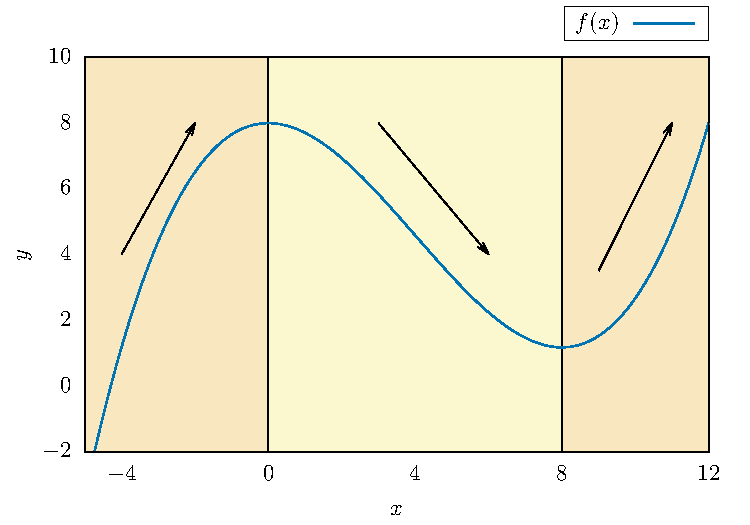
\includegraphics[scale = 0.7]{Gnuplot/Figures/funkce-rostouci-klesajici-obr.pdf}
    \caption{Ilustrace pojmu rostoucí a klesající funkce. Na oranžové oblasti je $f(x)$ rostoucí, na žluté oblasti je $f(x)$ klesající.}
\end{figure}

\begin{remark}
    Pokud mluvíme o růstu nebo poklesu funkce, je vždy nutné uvést, na jakém intervalu se pohybujeme. Důležitost je vidět na následujícím příkladu, viz obrázek \ref{fig:1a-funkce-ne}.

    \begin{figure}[H]
        \centering
        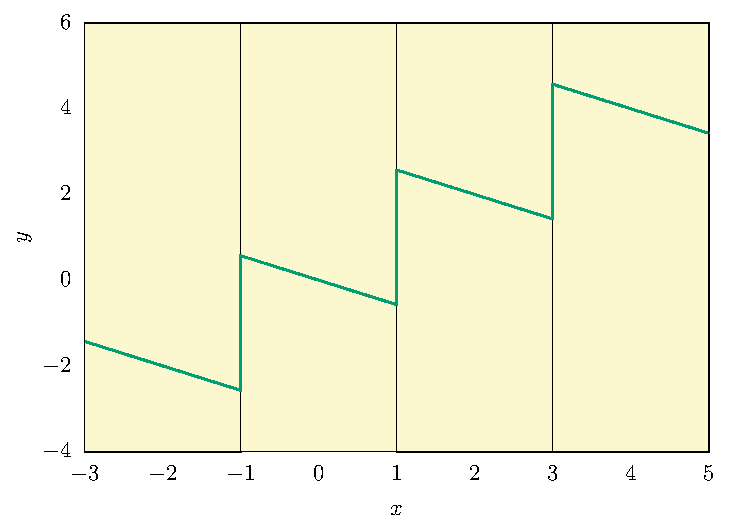
\includegraphics[scale = 0.7]{Gnuplot/Figures/periodicka-klesajici.pdf}
        
        \caption{Příklad funkce, která je klesající na každém intervalu $I_p = (2p-1,2p+1)$, kde $p \in \Z$. Na celém $\R$ ale není ani rostoucí, ani klesající. Porovnáme-li dva body $x_1 < x_2$ v témže intervalu $I_p$, splňují $f(x_1) > f(x_2)$. Porovnáme-li však body v různých intervalech, dostaneme $f(x_1) < f(x_2)$. Není tedy splněna ani jedna z podmínek pro růst nebo pokles na $\R$. Všimněme si, že funkce je v krajních bodech intervalů nespojitá, má v nich skoky.}
        \label{fig:1a-funkce-ne}
    \end{figure}

\end{remark}

\begin{remark}
    V některé literatuře se o různých křivkách mluví jako o \uv{rostoucích zleva doprava} nebo \uv{klesajících zprava doleva} a podobně. Matematická terminologie vždy pracuje s tím, co se děje s hodnotami $f(x)$ \underline{při rostoucích $x$} - tedy vždy \uv{zleva doprava}, chcete-li. Podobně se někdy říká o klesajících funkcích $y(x)$, že \uv{$y$ je nepřímo úměrné $x$}. Ale matematická terminologie říká, že pouze funkce $y(x)=C/x$ je nepřímá úměrnost, žádná jiná funkce toto nesplňuje.

    \begin{figure}[H]
        \centering
        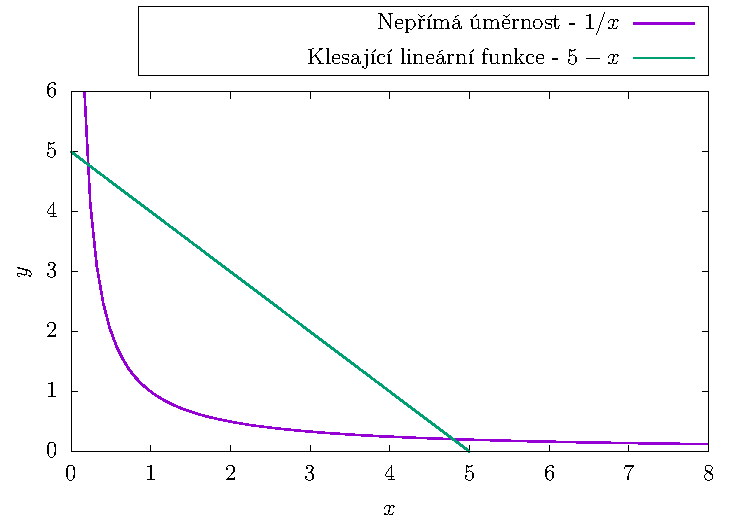
\includegraphics[scale = 0.7]{Gnuplot/Figures/neprima-umernost.pdf}
        \caption{Ilustrace často nesprávně použitého termínu \uv{nepřímá úměrnost}. Pouze funkce typu $C/x$ jsou nepřímé úměrnosti.}
    \end{figure}
\end{remark}

\subsection{Další charakteristiky funkce}

O funkci $f(x)$ říkáme, že je \begin{itemize}
    \item \textbf{prostá} na intervalu $I$, jestliže pro všechna $x,y \in I$ splňující $x \neq y$ platí $f(x) \neq f(y)$ (\uv{každému $x$ přísluší jiná hodnota $f(x)$}),
    \item \textbf{omezená shora}, jestliže existuje konečné číslo $K$ takové, že pro všechna $x \in D(f)$ platí $f(x) \leq K$,
    \item \textbf{omezená zdola}, jestliže existuje konečné číslo $K$ takové, že pro všechna $x \in D(f)$ platí $f(x) \geq K$,
    \item \textbf{omezená}, jestliže je omezená shora i zdola.
\end{itemize}

Jestliže je funkce $f$ prostá na intervalu $I$, pak k ní existuje \textbf{inverzní funkce}, kterou označujeme $f^{-1}$.

\begin{example}
    Funkce $x^2$ je prostá na intervalu $(-\infty, 0]$ a na intervalu $[0,+\infty)$. Není prostá na $\R$, protože $(-2)^2 = 4 = (+2)^2$.

    Na intervalu $[0,\infty)$ k ní existuje inverzní funkce $\sqrt{x}$. Na intervalu $(-\infty,0]$ k ní existuje inverzní funkce $\sqrt{-x}$.
\end{example}



\subsection{Příklady na definiční obor}

\begin{example}
    Určíme definiční obor funkce \begin{align*}
        R(x) = \frac{x^2-1}{(x+1)(x-4)(x^2 + 4x - 5)} \:.
    \end{align*}

    Řešení: První pravidlo nám říká, že nesmíme dělit nulou. Musíme tedy najít všechna $x$ taková, že je jmenovatel zlomku nulový: \begin{align*}
        (x+1)(x-4)(x^2 + 4x - 5) = 0 \:.
    \end{align*}
    Součin čísel (nebo výrazů, závorek) je nulový tehdy a jen tehdy, když je jedno z čísel nulové. Každou závorku tedy řešíme zvlášť:
    \begin{align*}
        \begin{cases}
            x+1 = 0 \Longrightarrow x = -1 \:, \\
        x-4 = 0 \Longrightarrow x = 4 \:, \\
        x^2 + 4x - 5 = 0 \Longrightarrow x = \frac{-4 \pm \sqrt{16+20}}{2} = - 2 \pm 3 \:, \: x = -5, 1
        \end{cases}
         \:.
    \end{align*}
    Tato řešení jsou body, které musíme z definičního oboru vyloučit. Tedy \begin{align*}
        \boxed{D(R) = \R \setminus \set{-5,-1,1,4} }\:.
    \end{align*}
    Poznámka: někdo by snad mohl postupovat tak, že by čitatel rovněž převedl na součin závorek: $x^2-1 = (x-1)(x+1)$. Jmenovatel lze též převést na součin: $x^2+4x-5 = (x+5)(x-1)$. Postupoval by tedy krácením:
    \begin{align*}
        R(x) = \frac{(x-1)(x+1)}{(x+1)(x-4)(x+5)(x-1)} \overset{?}{=} \frac{1}{(x+1)(x-4)} \:.
    \end{align*}
    Výraz na levé straně má jiný definiční obor: $\R \setminus \set{-1,4} \neq D(R)$.
    \textbf{Číselné hodnoty výrazů napravo a nalevo jsou stejné, ale definiční obor výrazů je různý!} Poučení tedy je: nejdříve nalezneme definiční obor a pak můžeme krátit.
\end{example}

\begin{example}
    Ještě jednou upozorníme na stejný případ: funkce $f(x) = \frac{x}{x}$ odpovídá konstantní funkci $g(x) = 1$, s tím rozdílem, že do $f$ nelze dosadit nulu. Takže \begin{align*}
        D(f) = \R \setminus \set{0} \neq \R = D(g) \:.
    \end{align*}
    
\end{example}

\begin{example}
    Určíme definiční obor funkce \begin{align*}
        h(x) = \sqrt{ \frac{\log (x-2)}{x-4}}
    \end{align*}

    Řešení: 1. pravidlo nám vyloučí bod $x=4$. 
    Dále nám 3. pravidlo říká, že do $\log$ můžeme dosadit pouze kladná čísla, takže musí platit $x-2>0$. To odpovídá hodnotám $x \in (2, \infty)$. 
    Konečně nám 2. pravidlo říká, že musí být výraz pod odmocninou nezáporný, musíme tedy řešit nerovnici \begin{align*}
        \frac{\log (x-2)}{x-4} \geq 0 \:.
    \end{align*}
    Nejprve vyřešíme případ, kdy platí rovnost.
    \begin{align*}
        \log (x-2) = 0 \Longrightarrow x-2 = 1 \Longrightarrow x = 3 \:.
    \end{align*}
    
    Nyní vyřešíme případ nerovnosti. Podíl dvou čísel je větší než nula právě tehdy, když jsou obě čísla kladná anebo obě čísla záporná (samozřejmě \uv{minus krát minus je plus}). Stačí tedy řešit podmínky:
    \begin{align*}
        \begin{cases}
            \left [\log (x-2) > 0 \right] \bigwedge \left[ x-4 > 0\right] \Longrightarrow [x \in (3,\infty)] \bigwedge [x \in (4, \infty)] \Longrightarrow x \in (4, \infty) \:, \\
            \left [\log (x-2) < 0 \right] \bigwedge \left[ x-4 < 0\right] \Longrightarrow [x \in (2,3)] \bigwedge [x \in (-\infty, 4)] \Longrightarrow x \in (2,3)
        \end{cases}
         \:.
    \end{align*}
    Celkově máme \begin{align*}
        \boxed{ D(h) = (2,3) \cup \set{3} \cup (4,\infty) = (2,3] \cup (4,\infty) } \:.
    \end{align*}
\end{example}

\begin{example}
    Určíme definiční obor funkce \begin{align*}
        P(x) = \frac{\arcsin (x-1)}{x^x} \:.
    \end{align*}

    Řešení: jmenovatel vyloučí bod nula. Dále, definiční obor funkce $\arcsin$ je $[-1,1]$, tedy $ -1 \leq x-1 \leq 1$, takže $x \in [0,2]$. 
    Nyní se podívejme na funkci ve jmenovateli. Tu můžeme přepsat \begin{align*}
        x^x = \left( e^{\log x} \right) = e^{x \log x} \:,
    \end{align*}
    takže se v ní objeví logaritmus a vidíme, že $x \in (0, \infty)$.
    Celkově \begin{align*}
        \boxed{ D(P) = [0,2] \cap (0, \infty) = (0,2] } \:.
    \end{align*}

\end{example}

\begin{example}
    Určíme definiční obor funkce 
    \begin{align*}
        m(t) = \tan (\sqrt{t+1}) \:.
    \end{align*}

    Řešení: odmocnina dává podmínku $t \in [-1,\infty)$. Dále platí $\tan x = \frac{\sin x}{\cos x} $, takže $\tan (\sqrt {t+1}) = \frac{\sin (\sqrt {t+1})}{\cos (\sqrt {t+1})}$. Protože nesmíme dělit nulou, musíme najít body \begin{align*}
        \cos (\sqrt{t+1}) = 0 \:.
    \end{align*}
    Substitucí $\sqrt{t+1} = u$ dostáváme podmínku $\cos u =0$, která odpovídá bodům $u = \frac{\pi}{2} + k \pi \:, k \in \Z$. Odtud máme \begin{align*}
        \sqrt{t+1} = \frac{\pi}{2} + k \pi \:.
    \end{align*}
    Nyní musíme vyjádřit $t$, což uděláme prostým umocněním a odečtením jedničky:
    \begin{align*}
        t =  \left( \frac{\pi}{2} + k \pi \right)^2 - 1 = \frac{\pi^2}{4} + 2 \cdot k \pi \cdot \frac{\pi}{2} + k^2 \pi^2 - 1 = k^2 \pi^2 + k \pi^2 + \frac{\pi^2}{4} - 1 \:.
    \end{align*}
    Definiční obor je tedy \begin{align*}
        D(m) = \set{t : t \geq -1, t \neq k^2 \pi^2 + k \pi^2 + \frac{\pi^2}{4} - 1, \: k \in \Z} \:.
    \end{align*}
\end{example}

\begin{example}
    Určíme definiční obor funkce \begin{align*}
        g(x) = \frac{\sin^3 x + 4^{-x}}{\sqrt{|2x-1|-|x+1|-3}} \:.
    \end{align*}
    Funkce v čitateli mají definiční obor $\R$. Musíme tedy zařídit, aby odmocnina ve jmenovateli byla dobře definovaná a aby byla nenulová, to znamená zajistit \begin{align*}
        |2x-1|-|x+1|-3 > 0 \:.
    \end{align*}

    Nerovnice s absolutní hodnotou se řeší pomocí tabulek. Nejprve najdeme body, kdy je absolutní hodnota nulová. V našem případě to jsou body $2x-1 = 0 \Rightarrow x=1/2$ a $x+1=0 \Rightarrow x=-1$. Nyní stačí využít toho, že $|x| = +x$ pro $x>0$ a $|x| = -x$ pro $x<0$.

    \begin{table}[H]
        \centering
        \begin{tabular}{c||c|c|c}
            
            \textbf{interval} & $(-\infty,-1)$ & $(-1,1/2)$ & $(1/2, +\infty)$ \\
            \hhline{=#=|=|=} 
            $|2x-1|$ & $-2x+1$ & $-2x+1$ & $+2x-1$ \\
            \hline
            $|x+1|$ & $-x-1$ & $+x+1$ & $+x+1$ \\
            \hhline{=#=|=|=}
            $|2x-1|-|x+1|-3$ & $(-2x+1)-(-x-1)-3$ & $(-2x+1)-(+x+1)-3$ & $(+2x-1)-(+x+1)-3$ \\
            \hline
            po úpravě & $-x-1$ & $ -3x - 3$ & $x-5$
            
        \end{tabular}
    \end{table}
    Nyní musíme vyřešit tři nerovnice \begin{align*}
        -x-1>0 \:, \quad -3x -3 >0 \:, \quad x-5 > 0 
    \end{align*}
    a podívat se, jestli spadají do zadaného intervalu.

    První rovnice odpovídá $x \in (-\infty,-1)$, což je v souladu s intervalem.
    Druhá rovnice odpovídá $x \in (-\infty,-1)$, který už není v souladu s intervalem.
    Třetí rovnice odpovídá $x \in (5, \infty)$, což je v souladu s intervalem.

    Celkově dostáváme 
    \begin{align*}
        \boxed{ D(g) = (-\infty, -1) \cup (5, \infty) } \:.
    \end{align*}
\end{example}

%\section*{Goniometrické a cyklometrické funkce}

\textbf{Goniometrické} (též trigonometrické) funkce jsou $\sin x$, $\cos x$, $\tg x$ a $\cotg x$. Funkce k nim inverzní, $\arcsin x$, $\arccos x$, $\arctg x$ a $\arccotg x$ nazýváme \textbf{cyklometrické}.

\subsubsection*{Arkussinus}

Graf funkce $\sin x$ je na obrázku \ref{fig:sinus}. Platí $D(\sin x) = \R$ a $H(\sin x) = [-1,1]$. Nyní potřebujeme vybrat interval, na kterém je tato funkce prostá, abychom k ní mohli nalézt inverzní. Zároveň chceme pokrýt \uv{co největší obor hodnot}. Nabízí se interval $[-\pi/2, \pi/2]$. Definujeme tedy funkci \textbf{arkussinus} $\arcsin x$ předpisem \begin{align}
    D(\arcsin x) = H(\sin x) = [-1,1] \:, \quad H(\arcsin x) = [-\pi/2, \pi/2] \:, \quad \arcsin(x) = y \Longleftrightarrow x = \sin y \:.
\end{align}

\begin{figure}[H]
    \centering
    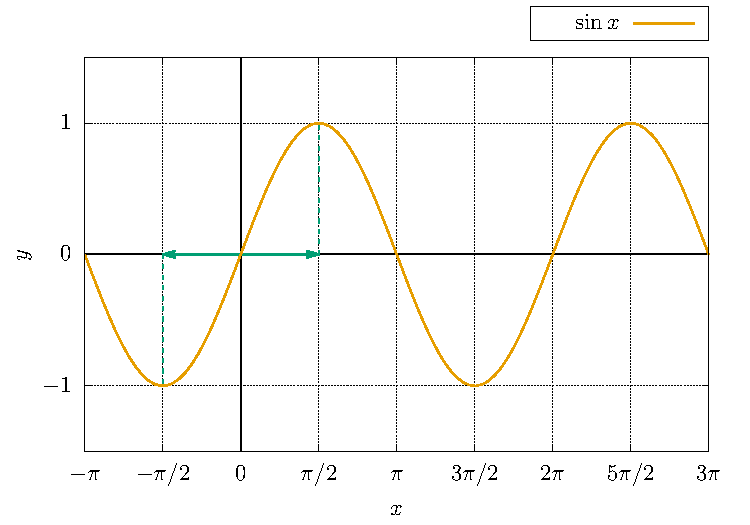
\includegraphics{Gnuplot/cv1/Figures/sinusgraf.pdf}
    \caption{Graf funkce sinus. Zeleně je vyznačen interval, kde je funkce prostá. Ten zvolíme jako obor hodnot funkce arkussinus.}
    \label{fig:sinus}
\end{figure}


\subsubsection*{Arkuskosinus}

Graf funkce $\cos x$ je na obrázku \ref{fig:kosinus}. Platí $D(\cos x) = \R$ a $H(\cos x) = [-1,1]$. Opět se chceme omezit na interval, kde je funkce prostá. Správný interval bude $[0,\pi]$. Definujeme funkci \textbf{arkuskosinus} $\arccos x$ předpisem \begin{align}
    D(\arccos x) = H(\cos x) = [-1,1] \:, \quad H(\arccos x) = [0, \pi] \:, \quad \arccos(x) = y \Longleftrightarrow x = \cos y \:.
\end{align}

\begin{figure}[H]
    \centering
    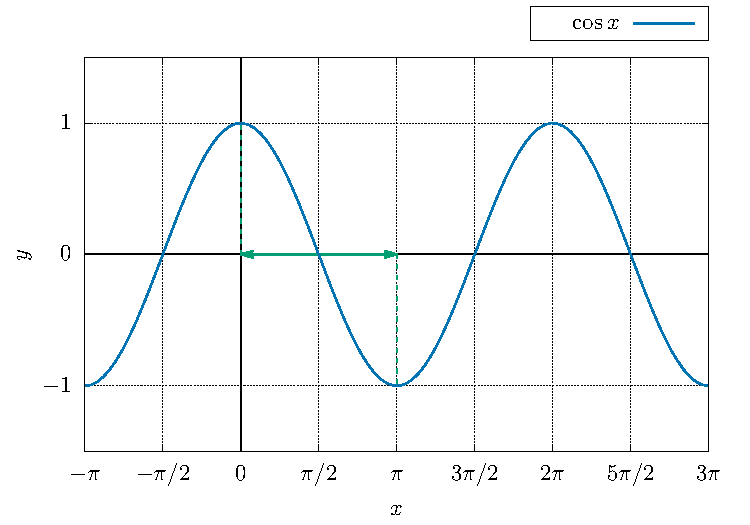
\includegraphics{Gnuplot/cv1/Figures/cosinusgraf.pdf}
    \caption{Graf funkce kosinus. Zeleně je vyznačen interval, kde je funkce prostá. Ten zvolíme jako obor hodnot funkce arkuskosinus.}
    \label{fig:kosinus}
\end{figure}

\subsubsection*{Arkustangens}

Graf funkce $\tg x$ je na obrázku \ref{fig:tangens}. Platí $D(\tg x) = \R \setminus \set{\frac{\pi}{2}+ k \pi, k \in \mathbb{Z}}$ a $H(\tg x) = \R$. Interval, na kterém je funkce prostá, je $(-\pi/2, \pi/2)$. Definujeme funkci \textbf{arkustangens} $\arccos x$ předpisem \begin{align}
    D(\arctg x) = H(\tg x) = \R \:, \quad H(\arctg x) = (-\pi/2, \pi/2) \:, \quad \arctan(x) = y \Longleftrightarrow x = \tg y \:.
\end{align}

\begin{figure}[H]
    \centering
    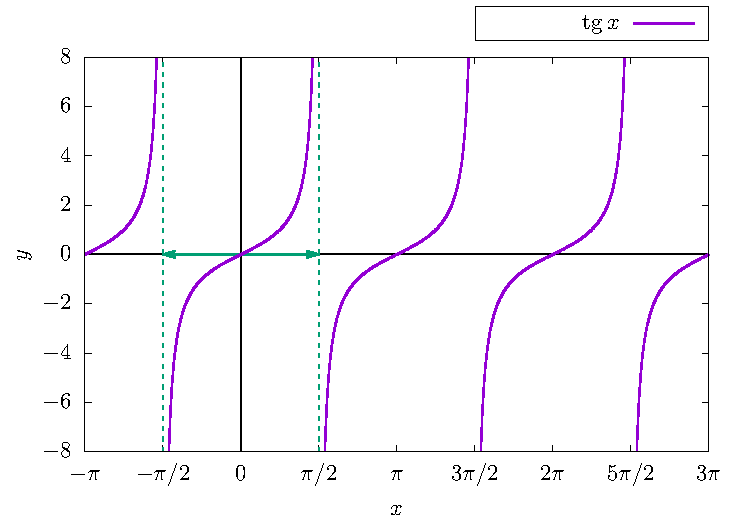
\includegraphics{Gnuplot/cv1/Figures/tangensgraf.pdf}
    \caption{Graf funkce tangens. Zeleně je vyznačen interval, kde je funkce prostá. Ten zvolíme jako obor hodnot funkce arkustangens. Povšimněme si, že v bodech $-\frac{\pi}{2}$ a $\frac{\pi}{2}$ jsou svislé asymptoty. Z nich se stanou vodorovné asymptoty funkce arkustangens.}
    \label{fig:tangens}
\end{figure}

\subsubsection*{Arkuskotangens}

Graf funkce $\cotg x$ je na obrázku \ref{fig:kotangens}. Platí $D(\cotg x) = \R \setminus \set{ k \pi, k \in \mathbb{Z}}$ a $H(\cotg x) = \R$. Interval, na kterém je funkce prostá, je $(0, \pi)$. Definujeme funkci \textbf{arkuskotangens} $\arccotg x$ předpisem 
\begin{align}
    D(\arccotg x) = H(\cotg x) = \R \:, \quad H(\arccotg x) = (0, \pi) \:, \quad \arccotg(x) = y \Longleftrightarrow x = \cotg y \:.
\end{align}

\begin{figure}[H]
    \centering
    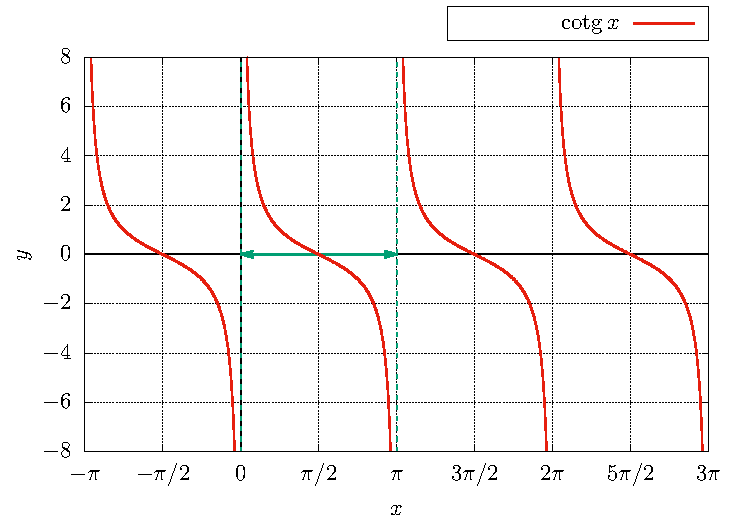
\includegraphics{Gnuplot/cv1/Figures/kotangensgraf.pdf}
    \caption{Graf funkce kotangens. Zeleně je vyznačen interval, kde je funkce prostá. Ten zvolíme jako obor hodnot funkce arkustangens. Povšimněme si, že v bodech $0$ a $\pi$ jsou svislé asymptoty. Z nich se stanou vodorovné asymptoty funkce arkuskotangens.}
    \label{fig:kotangens}
\end{figure}


Grafy funkcí $\arcsin x$ a $\arccos x$ jsou na obrázku \ref{obr:arcsin-arccos}, grafy $\arctg x$ a $\arccotg x$ jsou na obrázku \ref{obr:arctan-arccot}.

\begin{figure}[H]
    \centering
    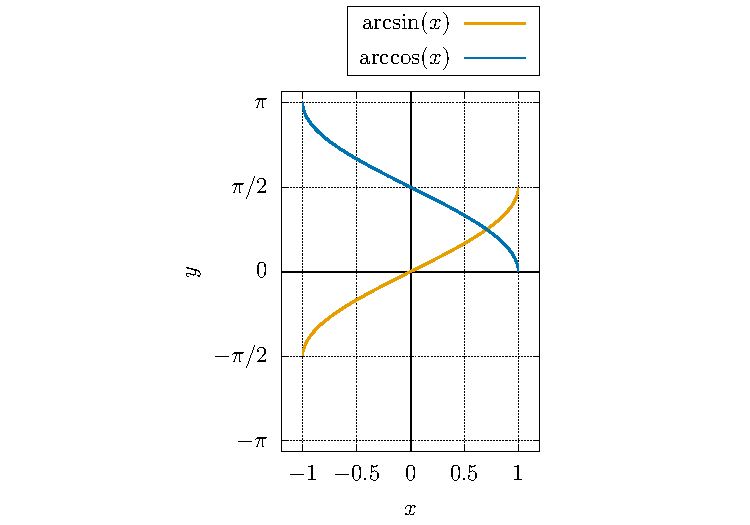
\includegraphics{Gnuplot/cv1/Figures/arcsin-arccos.pdf}
    \caption{Graf funkcí arkussinus a arkuskosinus.}
    \label{obr:arcsin-arccos}
\end{figure}
\begin{figure}[H]
    \centering
    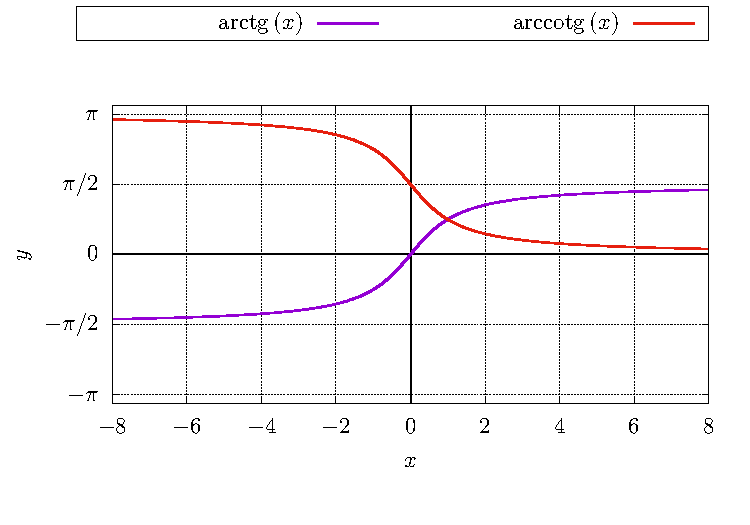
\includegraphics{Gnuplot/cv1/Figures/arctg-arccotg.pdf}
    \caption{Graf funkcí arkustangens a arkuskotangens.}
    \label{obr:arctan-arccot}
\end{figure}

%\subsection{Návod pro zobrazování grafů funkcí}

Existuje bezpočet placených i neplacených softwarů pro zobrazování funkcí. Jeden bezplatný lze nalézt na stránce \url{https://www.desmos.com/calculator}. Program umí počítat funkční hodnoty v jednotlivých bodech, sám vyznačí maxima a minima funkcí.

Pro symbol mocnění lze použít \fbox{\textsc{Ctrl+Alt+3}} ve Windows na české klávesnici, \fbox{\textsc{AltGr+M}} v Linuxu na české klávesnici, na anglické klávesnici \fbox{\textsc{Shift+6}}.
Pro zapsání zlomku stačí napsat \fbox{frac}, pro zapsání odmocniny \fbox{sqrt}. Symbol klávesnice dole na obrazovce umožní psát i složitější výrazy. Program rozlišuje přirozený \fbox{ln} a dekadický \fbox{log} logaritmus. 

Software si snadno poradí s funkcemi jedné proměnné, s implicitními funkcemi (typu $x^2+y^2=1$) a nerovnicemi.

Jeden ze silných nástrojů je posuvník. Pakliže do rovnice zadáme funkci s parametrem, můžeme vytvořit posuvník a sledovat, jak se se zvětšujícím nebo zmenšujícím parametrem mění její tvar.

\begin{exercise}[Lineární a kvadratická funkce]
    Až se dostaneme k pojmu derivace, budeme moci funkce aproximovat lineárními a kvadratickými funkcemi. Je velmi užitečné umět si takové funkce představit a vědět, kdy jsou rostoucí a klesající.
    \begin{enumerate}
        \item Zobrazte si lineární funkci $y(x) = px + q$ s posuvníky $p$ a $q$.
        \item Určete, pro která $p$ je funkce rostoucí, klesající a konstantní.
        \item Zjistěte, jakou roli hraje parametr $q$.
        \item Zobrazte si kvadratickou funkci $y(x) = ax^2 + bx +c$ s posuvníky $a,b,c$.
        \item Zjistěte, jakou roli hraje parametr $a$.
        \item Zjistěte, jakou roli hraje parametr $c$.
        \item Po kliknutí na graf funkce zobrazte minimum (maximum) a průsečíky s osami.
        \item Zkuste zjistit, jakou roli hraje parametr $b$. Co se děje s extrémem funkce?
    \end{enumerate}
\end{exercise}

\begin{exercise}[Gaussova křivka]
    V teorii pravděpodobnosti a statistiky je velmi důležitá tzv. Gaussova funkce (říká se jí též zvonová křivka, vlnový balík)
    \begin{align}
        f(x) = \frac{C}{\sqrt{2 \pi k^2}} \exp \left( - \frac{(x-m)^2}{2k^2}\right) \:.
    \end{align}
    Zobrazte si tuto funkci, měňte parametry $C$, $k$ a $m$. Zjišťujte, co se s funkcí děje.
\end{exercise}

\begin{exercise}[Příliš mnoho oscilací]
    Zobrazte funkci \begin{align}
        f(x) = \sin \left( \frac{1}{x} \right) \:.
    \end{align}
    Kolem počátku se nahrnuje příliš mnoho nulových bodů funkce. Zkuste je najít sami, tj. vyřešte rovnici $\sin(1/x) = 0$. 
    
    Funkce samozřejmě není definovaná v nule. V nějakém smyslu nabývá blízko nuly všech hodnot mezi $-1$ a $+1$. Vrátíme se k tomu, až budeme vyšetřovat limity funkcí. Tam si ukážeme, že $\sin(1/x)$ limitu v počátku nemá.
\end{exercise}
%\section{Aplikace první a druhé derivace}

\subsection{Lineární a kvadratická aproximace}

Hlavní význam derivací spočívá v tom, že pokud existují (říkáme, že funkce jsou \uv{dostatečně hladké}), můžeme pomocí nich funkce lokálně aproximovat.
Představme si funkci $f(x)$, která má první i druhou derivaci. Uvažujme nějaký \textbf{pevný bod $x_0$}. Na jeho \textbf{malém okolí} můžeme funkci aproximovat přímkou
\begin{align}
    \boxed{ T_1(x) = f(x_0) + f'(x_0) \cdot (x-x_0) }
\end{align}
nebo parabolou
\begin{align}
    \boxed{ T_2(x) = f(x_0) + f'(x_0) \cdot (x-x_0) +\frac{f''(x_0)}{2}  \cdot (x-x_0)^2 }\:.
\end{align}

\begin{example}
    Aproximujme funkci $f(x) = \sin(x)$ okolo bodu $x_0 = \pi/4$. Platí $f'(x) = \cos (x)$ a $f''(x) = - \sin (x)$, takže $f(\pi/4) = \sin (\pi/4) = \sqrt{2}/2$, $f'(\pi/4) = \cos (\pi/4) = \sqrt{2}/2$ a $f''(\pi/4) = - \sin (\pi/4) = -\sqrt{2}/2$.
    Na nějakém malém okolí tedy můžeme aproximovat přímkou \begin{align}
        T_1(x) = \frac{\sqrt{2}}{2} + \frac{\sqrt{2}}{2} \left(x - \frac{\pi}{4} \right)
    \end{align} 
    anebo parabolou
    \begin{align}
        T_2(x) = \frac{\sqrt{2}}{2} + \frac{\sqrt{2}}{2} \left( x - \frac{\pi}{4} \right) 
        - \frac{\sqrt{2}}{4} \left( x - \frac{\pi}{4} \right)^2  \:.
    \end{align}

    \begin{figure}[H]
        \centering

        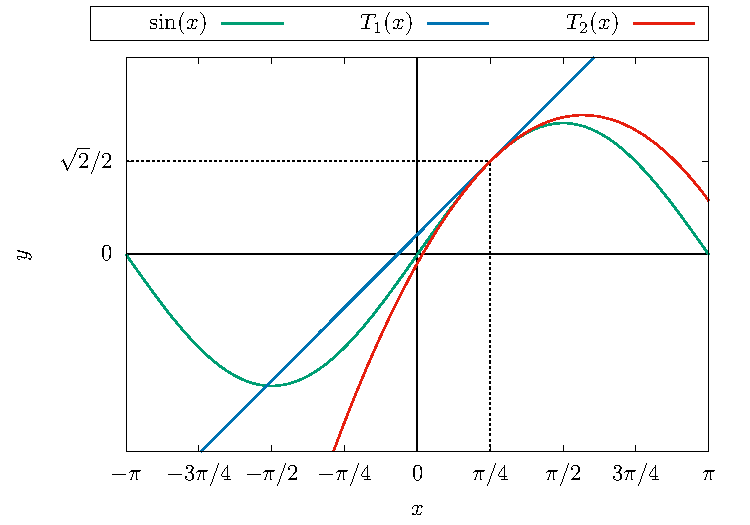
\includegraphics[scale = 0.7]{Gnuplot/Figures/aproximace-sinus.pdf}
        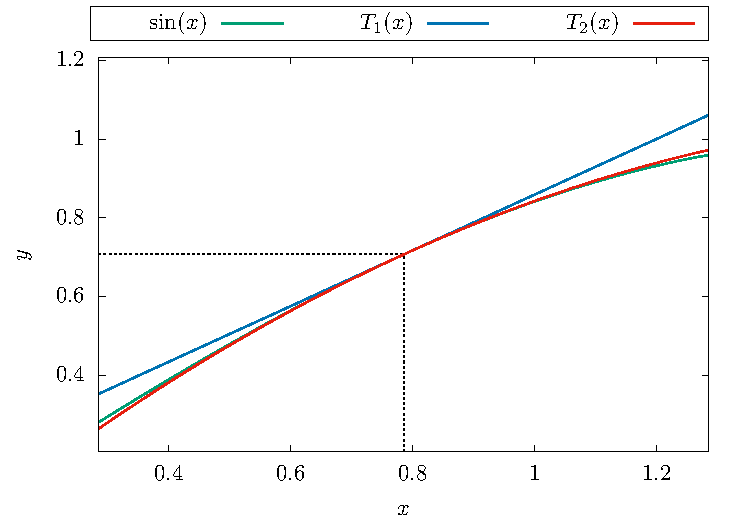
\includegraphics[scale = 0.7]{Gnuplot/Figures/aproximace-sinus2.pdf}

        \caption{Aproximace funkce $\sin x$ přímkou $T_1(x)$ a parabolou $T_2(x)$ kolem bodu $\frac{\pi}{4}$.}
    \end{figure}

\end{example}

\begin{example}
    Pomocí aproximace spočítejme $\sqrt{14}$. Víme, že $\sqrt{16} = 4$. Zkusme proto odmocninu aproximovat kolem bodu $4$. Platí \begin{align}
        (\sqrt{x})' = \frac{1}{2 \sqrt{x}} \:, \quad (\sqrt{x} )'' = -\frac{3}{2 \sqrt{x^3}} \:.
    \end{align}
    Můžeme tedy aproximovat parabolou \begin{align}
        \sqrt{x} \overset{\text{na okolí kolem }16} \approx \sqrt{16} + \frac{x-16}{2 \sqrt{16}}  -\frac{3(x-16)^2}{4 \sqrt{16^3}} = 4 + \frac{x-16}{8} - \frac{3(x-16)^2}{256}\:.
    \end{align}
    Nyní snadno spočteme \begin{align}
        \sqrt{14} = 4 - \frac{2}{8} - \frac{8}{256} = 3,72 \:.
    \end{align}
    V porovnání se skutečnou hodnotou $\sqrt{14} = 3,7416$ vidíme, že jsme se o spletli o pouhých $6$ promile.
\end{example}

Můžeme samozřejmě pokračovat a rozvíjet funkce do tzv. \textbf{Taylorovova polynomu} $T_n(x)$ pomocí vyšších a vyšších derivací. Nicméně to ve většině praktických případů není příliš potřeba, bohatě si vystačíme s parabolickou aproximací $T_2(x)$.

\subsection{Rostoucí, nebo klesající?}

Podle lineární aproximace $T_1(x)$ snadno poznáme, jestli je funkce na daném okolí rostoucí nebo klesající. V aproximaci totiž \textbf{$f'(x_0)$ zastupuje lineární koeficient přímky}. Je-li tedy $f'(x_0)>0$, pak se jedná o rostoucí lineární aproximaci a tedy i o rostoucí funkci. Obdobně, je-li $f'(x_0) <0$, pak je aproximace klesající přímka a funkce je jistě klesající.

\subsection{Minimum a maximum}

Z rozvojů $T_1(x)$ a $T_2(x)$ také snadno můžeme rozpoznat minimum a maximum funkce. 
Jestliže je nějaký bod $x_0$ extrémem funkce $f(x)$, pak musí být $f'(x_0)=0$, protože jinak bychom měli lineární aproximaci $T_1(x)$ s nenulovou směrnicí, tj. rostoucí nebo klesající přímku. To znamená, že nějaký bod na okolí by měl jistě nižší anebo vyšší funkční hodnotu, takže by bod $x_0$ jistě nebyl extremální. \textbf{Chceme-li tedy hledat minimum a maximum hladkých funkcí, jedinými kandidáty jsou tzv. stacionární body, tj. body $x_0$, ve kterých je $f(x_0)$.} 

Teď se podívejme na kvadratický rozvoj $T_2(x)$. Jestliže $f'(x_0)=0$ a $f''(x_0) > 0$, pak se jedná o parabolu 
\begin{align}
    T_2(x) = f(x_0) + \frac{1}{2} f''(x_0) (x-x_0)^2
\end{align}
s kladným kvadratickým koeficientem, takže bude \uv{typu $\cup$}. Tím pádem je v $x_0$ minimum, protože parabola od něj \uv{roste napravo i nalevo}.

Podobně, představme si, že $f''(x_0) < 0$. Pak se jedná o parabolu \uv{typu $\cap$} a $x_0$ tedy musí být maximum, protože parabola \uv{napravo i nalevo klesá}.

\subsection{Konkavita, konvexita, inflexní bod}

Matematická definice těchto pojmů je složitější, nicméně se dají názorně představit. Uvažujme funkci $f$ a nějaké dva libovolné body $x_1$ a $x_2$. Představme si, že spojíme body na grafu $[x_1, f(x_1)]$ a $[x_2, f(x_2)]$ úsečkou.
\textbf{Jestliže celá tato úsečka leží nad grafem funkce, nazývá se funkce konvexní. Jestliže leží úsečka celá pod grafem funkce, nazývá se funkce konkávní.}

Představíme-li si paraboly $x^2$ a $-x^2$, pak je jasné, že $x^2$ je konvexní a $-x^2$ je konkávní. U parabol tedy o konkávitě nebo konvexitě rozhoduje znaménko kvadratického koeficientu.

Ale my již víme, že i složitější funkce umíme kvadraticky aproximovat do paraboly $T_2(x)$ s kvadratickým koeficientem $f''(x_0)$. Jestliže je tedy $f''(x_0)>0$, pak je jistě funkce konkávní, jestliže je $f''(x_0)<0$, pak je funkce konvexní.

\textbf{Inflexní bod je takový, kde $f''(x_0) = 0$.} Tam žádný kvadratický koeficient není a funkce se lokálně chová jako obyčejná přímka.

\subsection{Sedlový bod}

Může samozřejmě nastat případ, kdy najdeme stacionární bod $x_0$ splňující nejen $f'(x_0)$, ale i $f''(x_0) = 0$. V takovém případě nemůžeme pomocí tohoto přístupu rozhodnout, zda se jedná o minimum, maximum, nebo sedlový bod. Sedlový bod je takový, kde se lokálně funkce chová jako konstanta, ale nejedná se ani o minimum nebo maximum.

\begin{example}
    Funkce $g(x)=x^3$ má zjevně stacionární bod $x_0 = 0$. V tomto bodě první i druhá derivace $g$ jsou rovny nule. Jedná se o sedlový bod, ale to \uv{na papíře} nepoznáme, pokud nepoužijeme nějaké další techniky. (Samozřejmě to ihned poznáme z grafu.)
\end{example}

\subsection{Shrnutí}

\begin{figure}[H]
    \centering
    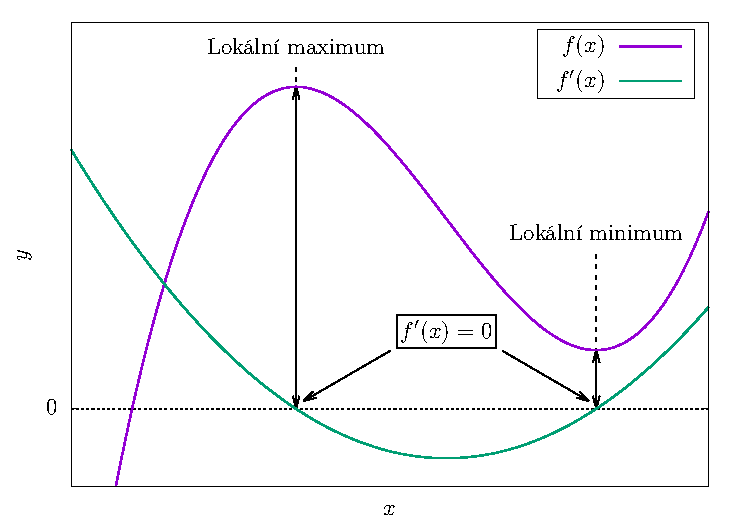
\includegraphics[scale = 0.7]{Gnuplot/Figures/funkce-derivace.pdf}
    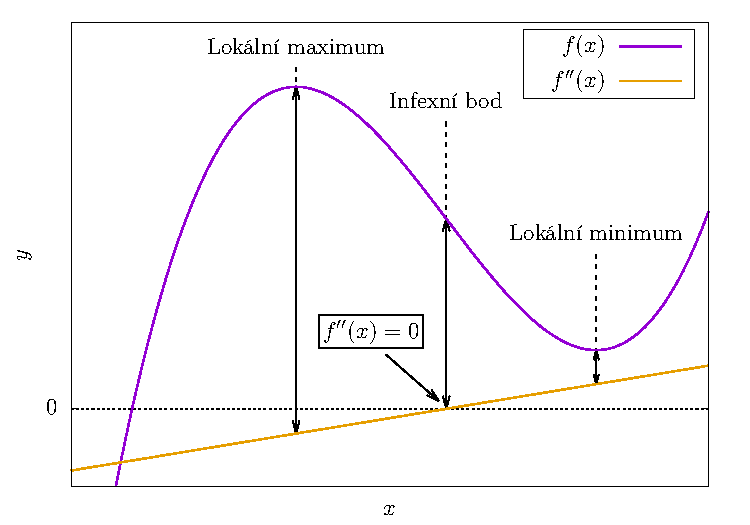
\includegraphics[scale = 0.7]{Gnuplot/Figures/funkce-druha-derivace.pdf}
    \caption{Ilustrace průběhu funkce, její první a druhé derivace.}
\end{figure}
\begin{table}[H]
    \centering

    \begin{tabular}{|c|c|c|}
        \hline
        vlastnost funkce & první derivace & druhá derivace \\
        \hline
        rostoucí & $+$ & jakákoli \\
        klesající & $-$ & jakákoli  \\
        konvexní & jakákoli & $+$ \\
        konkávní & jakákoli & $-$ \\ \hline
    \end{tabular}
    \caption{Charakterizace funkce podle první a druhé derivace.}
\end{table}

\begin{table}[H]
    \centering

    \begin{tabular}{|c|c|c|}
        \hline
        speciální bod & první derivace & druhá derivace \\
        \hline
        lokální minimum & $0$ & $+$ \\
        lokální maximum & $0$ & $-$ \\
        sedlový bod & $0$ & $0$ \\
        inflexní bod & jakákoli & $0$ \\ \hline
    \end{tabular}
    \caption{Charakterizace speciálních bodů funkcí. U sedlového bodu nejsou podmínky postačující.}
\end{table}

\section{Příklady}

\begin{example}
   

\end{example}

\section{Aplikované příklady}

\begin{example}[Maximální profit]
    Dejme tomu, že náklady $TC$ na výrobu produktu o množství $Q$ jsou dány funkcí 
    \begin{align}
        TC (Q) = 2 Q^3 - 3 Q^2 + 400 Q + 5000 
    \end{align}
    a cena produktu $P$ je dána funkcí \begin{align}
        P(Q) =  4000 - 33 Q \:.
    \end{align}
    Profitová funkce $\Pi$ (čti \uv{velké pí}) je dána rozdílem celkového příjmu a celkového nákladu
    \begin{align}
        \Pi = TR - TC \:, \quad \text{kde} \quad TR = P \cdot Q \:.
    \end{align} 
    Určeme maximální profit.

    Platí \begin{align}
        \Pi(Q) = 4\,000 Q - 33 Q^2 - 2 Q^3 + 3 Q^2 - 400 Q - 5\,000 = - 2 Q^3 - 30 Q^2 + 3\,600 Q - 5\,000\:.
    \end{align}
    Naším úkolem je nalézt maxima a minima takové funkce. K tomu spočteme derivaci
    \begin{align}
        \Pi'(Q) = - 6Q^2 - 60 Q + 3\,600
    \end{align}
    a určíme její nulové body $Q_0$. Musíme tedy vyřešit rovnici 
    \begin{align}
        Q_0^2 + 10 Q_0 - 600 = 0\:,
    \end{align}
    což není žádný problém:
    \begin{align}
        Q_0 = \frac{-10 \pm \sqrt{100 + 2\,400}}{2} = - 5 \pm 25 = -30 \:, \: +20 \:. 
    \end{align}
    Zjevně nás zajímá bod $Q_0 = 20$. Pomocí druhé derivace ověříme, o jaký stacionární bod se jedná.
    \begin{align}
        \Pi''(Q) = - 12 Q - 60 \:, \quad \Pi''(Q_0) = - 12 \cdot 20 - 60 < 0 \:,
    \end{align}
    takže se jedná o lokální maximum.

    Maximální profit tedy nastává při množství $Q_0 = 20$ a je roven 
    \begin{align}
        \Pi_{\text{max}} 
    = \Pi(Q_0) = -2 \cdot 20^3 - 30 \cdot 20^2 + 3600 \cdot 20 - 5\,000 = 39\,600 \:.
    \end{align}
\end{example}
%\section{Diferenciální rovnice}

Rovnice tvaru \begin{align}
    F(x,y(x),y'(x),\cdots, y^{(n)}(x)) = 0 \:,
\end{align}
kde $y(x)$ je neznámá funkce, se nazývá \textbf{obyčejná diferenciální rovnice} $n$-tého řádu.

Rovnice tvaru \begin{align}
    F(\vc x, y(\vc x), \DD^\lambda y(\vc x)) \:,
\end{align}
kde $\vc x = (x_1, \cdots, x_n) \in \R^n$, $y(\vc x)$ je neznámá funkce $n$ proměnných a $\DD^\lambda$ označuje její parciální derivace, se nazývá \textbf{parciální diferenciální rovnice}.


Je snad na tomto místě vhodné zdůraznit, že diferenciální rovnice se svou povahou naprosto liší od rovnic lineárních, kvadratických, exponenciálních a podobně. Hledat neznámé funkce je totiž řádově těžší, než hledat obyčejná čísla. Proč? Pro většinu algebraických rovnic máme numerické metody, které jsou dnes velmi přesné a rychlé. Navíc máme většinou záruku, že existují. Řešení obyčejných diferenciálních rovnic (a hlavně jejich soustav) je zpravidla nemožné nalézt analyticky a časová náročnost řešení numericky je daleko větší. Nejhůře na tom jsou parciální diferenciální rovnice, o nich často nevíme, zda vůbec nějaké řešení mají, a pokud ho mají, je velmi obtížné ho hledat numericky. Kdybychom to uměli rychle, mohli bychom lépe porozumět mnoha jevům v mnoha vědeckých oblastech: například bychom porozuměli turbulencím, stavěli kvantové počítače, mohli bychom přesně předpovídat počasí i situaci na trhu na měsíce dopředu, projektovali bychom stavby, které by přežily tisíciletí, \dots

\begin{table}[H]
    \centering
    \begin{tabular}{c|c|c}
        Typ rovnice & Neznámý objekt & Náročnost (na stupnici $1-10$) \\
        \hline
        lineární & jediné číslo $x$ & $1$ \\
        kvadratická & dvě čísla $x_{1,2}$ & $2$ \\
        algebraická (jakkoli ošklivá) & jedno nebo několik čísel $x_k$ & $3-5$ \\
        \hline
        obyčejná diferenciální (bez podmínek) & soubor funkcí $\set {y_\lambda(x)}$ & $8+$ \\
        obyčejná diferenciální (s počáteční podmínkou) & jediná funkce $y(x)$ & $8$ \\
        obyčejná diferenciální (s okrajovou podmínkou) & jediná funkce $y(x)$ & $10+$ \\
        \hline
        parciální diferenciální (s podmínkou či bez) & funkce více proměnných $y(x_1, \cdots, x_N)$ & $20+$
    \end{tabular}
\end{table}

Diferenciální rovnice typicky řešíme na nějaké vybrané množině a můžeme je doplnit o takzvané počáteční nebo okrajové podmínky. Řešením rovnic bez podmínek jsou soubory (množiny, třídy, \dots) funkcí.

\subsection{Lineární diferenciální rovnice}

Nejjednodušší diferenciální rovnice jsou lineární diferenciální rovnice 
\begin{align}
    a_n(x) y^{(n)}(x) + a_{n-1}(x) y^{(n-1)}(x) + a_{n-2}(x) y^{(n-2)}(x) + \cdots + a_1(x) y(x) = f(x) \:,
\end{align}
kde $y(x)$ je neznámá funkce, $a_k(x)$ a $f(x)$ jsou známé funkce.

Lineární se jim říká proto, že se tak trochu chovají jako vektory. Součet dvou různých řešení je zase řešení. Stejně tak libovolný násobek řešení je zase řešení.

Ještě jednodušší jsou rovnice, kde funkce $a_k(x)$ jsou pouhé konstanty. Těm se říká rovnice s konstantními koeficienty:
\begin{align}
    c_n y^{(n)}(x) + c_{n-1} y^{(n-1)}(x) + c_{n-2} y^{(n-2)}(x) + \cdots + c_1 y(x) + a_0 = f(x) \:.
\end{align}
My se naučíme řešit lineární diferenciální rovnice druhého řádu s konstantními koeficienty 
\begin{align}
    a y''(x) + b y'(x) + c y(x) = f(x) \:.
\end{align}

\subsection{Homogenní (zkrácená) rovnice}

Začneme s řešením rovnic, které na pravé straně obsahují nulu, tj. \begin{align}
    a y''(x) + b y'(x) + c y(x) = 0 \:.
\end{align}
Tuto rovnici vždy totiž řeší exponenciální funkce $y(x) = e^{\lambda x}$ pro nějaké konkrétní $\lambda$, které nyní určíme. Zkusme tuto funkci do rovnice dosadit. Dostaneme
\begin{align}
    a (e^{\lambda x})'' + b (e^{\lambda x})' + c = a \lambda^2  e^{\lambda x} + b \lambda e^{\lambda x} + c e^{\lambda x} = e^{\lambda x} [a \lambda^2 + b \lambda + c ] = 0 \:.
\end{align}
Součin bude roven nule právě tehdy, když hranatá závorka bude nule. Tím jsme dostali obyčejnou algebraickou rovnici \begin{align}
    a \lambda^2 + b \lambda + c = 0 \:.
\end{align}
Tato rovnice má obecně dvě řešení v oboru komplexních čísel $\C$. Je potřeba rozlišit tři případy:
\begin{enumerate}
    \item Oba kořeny $\lambda_1$, $\lambda_2$ jsou různé a reálné. Pak je řešení homogenní rovnice \begin{align}
        y(x) = C_1 e^{\lambda_1 x} + C_2 e^{\lambda_2 x} \:,
    \end{align}
    kde $C_1$ a $C_2$ jsou \textbf{libovolné volitelné koeficienty} (vzpomeňme si, že součet dvou řešení a číselný násobek řešení je zase řešení).

    \item Získáme-li dvojnásobný kořen $\lambda_1 = \lambda_2 := \lambda $, pak je řešení homogenní rovnice \begin{align}
        y(x) = (Ax + B) e^{\lambda x } \:,
    \end{align}
    kde $A$ a $B$ jsou opět volitelné koeficienty.

    \item Získáme-li komplexně sdružené kořeny $\lambda_{1,2} = p \pm i q$, pak je řešení homogenní rovnice \begin{align}
        y(x) = e^{px} \left( C_1 \sin (q x) + C_2 \cos(qx) \right) \:,
    \end{align}
    kde $C_1$ a $C_2$ jsou volitelné koeficienty.
\end{enumerate}

\begin{example}[Množení populace]
    Uvažujme populaci (např. bakterií), jejíž jedinci neumírají a stále se množí.
    Populace v čase bude narůstat tím víc, čím více obsahuje jedinců. To matematicky můžeme vyjádřit vztahem
    \begin{align}
        \dder{P}{t} = k P(t) \:, \quad k > 0 \:.
    \end{align} 
    Zkusme tedy vyřešit diferenciální rovnici $P'(t) = k P(t)$ a podívat se, za jak dlouho populace vzroste na desetinásobek.

    Charakteristická rovnice je $\lambda - k = 0$, odtud $\lambda = k$. Řešení této rovnice je tedy $P(t) = C e^{k t} $, kde $C$ je nějaká konstanta.

    Předpokládejme nyní, že v čase $t=0$ obsahuje populace $P_0$ jedinců. Abychom tuto podmínku splnili, stačí dosadit do řešení nulu:
    \begin{align}
        P(0) = C e^{k \cdot 0} = P_0 \:, \quad \text{takže} \quad C = P_0
    \end{align}
    a máme řešení
    \begin{align}
        P(t) = P_0 e^{kt} \:.
    \end{align}
    Populace se bude množit exponenciálně! Za jaký čas $t_{10}$ vzroste populace na $10 P_0$? Stačí vyřešit rovnici 
    \begin{align}
        10 P_0 = P(t_{10}) = P_0 e^{k t_{10}} \:.
    \end{align}
    Její řešení je $t_{10} = \frac{1}{k} \log (10) \approx \frac{2,30}{k}$. Čím větší bude $k$, tím rychleji se populace bude množit.
\end{example}

\subsection*{Závěrečné poznámky}

\begin{itemize}
    \item Řešení diferenciálních rovnic nemusí být jednoznačné ani při zadání konkrétní počáteční podmínky. Například rovnici 
    \begin{align}
        y'(x) = \frac{1}{3} \sqrt[3]{y(x)}  \:, \quad \text{s počáteční podmínkou } y(0) = 0
    \end{align}
    řeší jak funkce $y(x) = (2 x)^{3/2}$, tak $y(x) = 0$. Tomuto jevu se říká \textbf{bifurkace} a je velmi důležité ho zkoumat, např. při konstrukci laseru nebo nanočipů.

    \item Někdy malá změna počátečních podmínek vede ke kvalitativní změně řešení (řešení se začne chovat úplně jinak). Například rovnice
    \begin{align}
        y'(x) = 1 - y^2(x)
    \end{align}
    řeší pro podmínku $y(0) = -1$ konstantní funkce $y(x) = -1$. Změníme-li ale počáteční podmínku o chloupeček, řekněme na $y(0) = -0.999$, pak dostaneme řešení, která buďto rostou do $+1$ anebo utíkají z minus nekonečna.

    Tento jev se nazývá \textbf{efekt motýlích křídel} (butterfly effect) a je zodpovědný za to, že nemůžeme přesně předpovědět počasí na více než dva dny dopředu (\uv{zamávání křídla motýla v Texasu vyvolá tornádo v Číně}). Máme sice správné rovnice (a umíme je řešit), ale kvůli nepřesné znalosti počátečních podmínek (tlaku vzduchu, teploty, složení ovzduší, atd\dots) si nemůžeme být jisti, která varianta nastane. Podobný problém samozřejmě nastává i u předpovědí finančního trhu, chování společnosti a dokonce i u solárního systému (stále nevíme s jistotou, zda je naše Sluneční soustava stabilní - přitáhne nás jednoho krásného dne Jupiter?). Obecněji se těmito problémy zabývá \textbf{teorie chaosu} a teorie \textbf{fraktálů}. Více lze nalézt např. ve výborné, populárně naučné knížce \textsc{Hraje bůh kostky?} od Iana Stewarta.

    \item Řešení \href{https://en.wikipedia.org/wiki/Navier%E2%80%93Stokes_equations}{jedné parciální diferenciální rovnice} bylo zařazeno mezi 
    \href{https://en.wikipedia.org/wiki/Millennium_Prize_Problems}{Sedm problémů tisíciletí}. Tento problém (jeho formulace) je ze všech nejjednodušší na pochopení. Odměna za jeho řešení je jeden milion dolarů! Stále není pozdě připojit se k matematikům a pokračovat v jejich marném celoživotním boji. Motivací ale nejsou peníze, jak dokládá \href{https://www.youtube.com/watch?v=vNcarnNJPqs}{Grigorij Perelman, který jeden z těchto problémů vyřešil}.

    \item Další důležitá třída rovnic jsou tzv. \textbf{diferenční rovnice}, jejichž cílem je nalézt z předpisu \begin{align}
        F(n, a_n, a_{n-1}, \cdots , a_{n-k}) = 0
    \end{align}
    neznámou posloupnost $\set{a_n}$. Typickým příkladem je rovnice \begin{align}
        a_{n} = a_{n-1} + a_{n-2} \:, \quad a_0 = a_1 = 1 \:,
    \end{align}
    jejímž řešením jsou Fibonacciho čísla $1,1,2,3,5,8,13,21,34,55,\cdots$. Náročnost diferenčních rovnic je pro člověka zhruba stejná jako náročnost diferenciálních, nicméně počítače je řeší mnohem snáze. Hodí se například k počítání úroků. 

    \item 
\end{itemize}


%\section{Průběh funkce}



\subsection{Kuchařka pro vyšetřování průběhu funkce}

\begin{enumerate}

    \item Určíme definiční obor $D(f)$.
    
    \item Zkusíme zjistit, zda je funkce symetrická:
    \begin{itemize}
        \item Pro sudou funkci platí $f(x) = f(-x)$.
        \item Pro lichou funkci platí $-f(x) = - f(-x)$.
    \end{itemize}

    \item Spočítáme průsečíky funkce s osami $P_x$ a $P_y$:
    \begin{itemize}
        \item Bod $P_x$ nalezneme řešením rovnice
        $f(x)=0$.
        \item Bod $P_y$ nalezneme prostým dosazením bodu $0$ do funkce, tj. spočteme $f(0)$.
    \end{itemize}
     
    \item Určíme limity v bodech nespojitosti funkce a limity v bodech $\pm \infty$ (pokud existují).

    \item Vyšetříme lokální minima a maxima:
    \begin{itemize}
        \item Spočteme $f'(x)$, $f''(x)$ a najdeme stacionární body $x_0$, které odpovídají rovnici $f'(x_0) = 0$.
        \item Jestliže $f''(x_0) < 0$, pak má $f$ v $x_0$ lokální maximum.
        \item Jestliže $f''(x_0) > 0$, pak má $f$ v $x_0$ lokální minimum.
        \item Nalezneme funkční hodnoty $f(x_0)$, případně je mezi sebou porovnáme.
    \end{itemize}
    
    \item Nalezneme inflexní body řešením rovnice $f''(x_{\text{flex}}) = 0$.
    
    \item Určíme intervaly, na kterých $f'(x)$ a $f''(x)$ nemění znaménko.
    \begin{itemize}
        \item Na intervalu, kde platí $f'(x) > 0$, je $f$ rostoucí.
        \item Na intervalu, kde platí $f'(x) < 0$, je $f$ klesající.
        \item Na intervalu, kde platí $f''(x) > 0$, je $f$ konvexní.
        \item Na intervalu, kde platí $f''(x) < 0$, je $f$ konkávní.
    \end{itemize}

    \item Někdy můžeme vyšetřovat asymptotické chování funkce.
    \begin{itemize}
        \item Lineární asymptoty jsou přímky $u(x) = px+q$, kde 
        \begin{align*}
            p = \lim_{x \rightarrow \pm \infty} \frac{f(x)}{x} \quad \text{a} \quad q = \lim_{x \rightarrow \pm \infty} f(x) - px \:.
        \end{align*}
        Samozřejmě nemusí existovat.
        \item Můžeme také limitní chování porovnávat s mocninnými funkcemi typu $x^\alpha$, tj. nalézt takové $\alpha$, aby \begin{align*}
            \lim_{x \rightarrow \pm \infty} \frac{f(x)}{x^\alpha} \quad \text{byla vlastní a nenulová} \:.
        \end{align*}
        V takovém případě pak píšeme $f(x) = O(x^\alpha)$ pro $x \rightarrow \pm \infty$.
    \end{itemize}

    \item Nakreslíme graf funkce $f(x)$.
\end{enumerate}

\begin{example}
    Vyšetříme průběh funkce $f(x) = \frac{x^2-1}{x^2-5x+6}$.

\begin{enumerate}
    \item Definiční obor funkce: jmenovatel nesmí být nulový, tedy řešíme rovnici $x^2-5x +6 = 0$. Jejím řešením jsou body $3$ a $2$, tedy \begin{align*}
        D(f) = \R \setminus \set{3,2} \:.
    \end{align*}

    \item Funkce zjevně není ani symetrická, ani antisymetrická.
    \item Průsečík s osou x: řešíme rovnici $x^2-1 = 0$. Řešením jsou body $\pm 1$.
    Průsečík s osou y: stačí spočítat $f(0) = -\frac{1}{6} $.
    Průsečíky jsou tedy \begin{align*}
        P_x^{(1)} = [-1;0] \:, \quad P_x^{(2)} = [1;0] \:, \quad P_y = [0;-1/6] \:.
    \end{align*}
    \item Určíme limity funkce v $\pm \infty$:
    \begin{align*}
        \lim_{x \rightarrow + \infty} \frac{x^2-1}{x^2-5x+6} = 1 \:, \quad \lim_{x \rightarrow - \infty} \frac{x^2-1}{x^2-5x+6} = 1 \:.
    \end{align*}
    Také nesmíme zapomenout na limity v bodech nespojitosti:
    \begin{align*}
        \lim_{x \rightarrow 2_-} \frac{x^2-1}{x^2-5x+6} 
        =+ \infty \:, 
        \quad 
        \lim_{x \rightarrow 2_+} \frac{x^2-1}{x^2-5x+6} 
        = - \infty \:, \\
        \lim_{x \rightarrow 3_-} \frac{x^2-1}{x^2-5x+6} 
        = - \infty \:,
        \quad 
        \lim_{x \rightarrow 3_+} \frac{x^2-1}{x^2-5x+6} 
        = + \infty \:.
    \end{align*}
\end{enumerate}
\end{example}










%%-------------------------------------
%	BIBLIOGRAPHY
%-------------------------------------

\renewcommand{\refname}{\spacedlowsmallcaps{References}} % For modifying the bibliography heading

\bibliographystyle{unsrt}

\bibliography{sample.bib} % The file containing the bibliography

%------------------------------------

\end{document}